% ============================================================
% Section 4: Performance Evaluation
% ============================================================

\section{Performance Evaluation}
\label{sec:evaluation}

In this section, we evaluate the impact of the proposed Preemptive scheduling method
on the campus GPU sharing platform Air Computing Pool (ACP)
through a discrete-event simulation.
The evaluation proceeds in four steps.
First, we describe the simulation setup.
Second, we show that sharing improves overall TAT but that existing policies
harm high-performance GPU owners at high load.
Third, we demonstrate that Preemptive is the only policy that guarantees
owner protection and thereby sustains participation equilibrium.
Finally, we verify this result holds across diverse workload distributions.

% \section{性能評価}
% \label{sec:evaluation}
%
% 本章では，提案するプリエンプティブ方式が学内GPU共有基盤ACPに与える影響を，
% 離散イベントシミュレーションにより評価する．評価は以下の4段階で進める．
% まずシミュレーション環境を説明し，
% 次に共有がTATを全体的に改善する一方で既存方式が高性能GPU所有者を高負荷時に不利にすることを示す．
% そのうえで，プリエンプティブ方式のみが所有者保護を保証してシステムの持続的平衡を実現することを示す．
% 最後に，この結果が多様なワークロード分布でも成立することを検証する．

% ============================================================
\subsection{Simulation Environment}
\label{sec:sim_env}
% ============================================================

We constructed a discrete-event simulation of a campus GPU sharing environment
consisting of 18 users.
Each user owns one GPU categorized into one of nine performance tiers,
with two users per tier.
GPU throughput values are based on real FP16 Tensor FLOPS,
ranging from GTX 1650 (2.98 TFLOPS) to A100 (311.84 TFLOPS) (Table~\ref{tab:gpu_tiers}).
The performance ratio between the lowest and highest tiers is approximately 105$\times$,
reflecting the wide heterogeneity typical of campus environments
where researchers acquire GPUs at different points in time.

% \subsection{シミュレーション環境}
% \label{sec:sim_env}
%
% 本研究では，18ユーザーで構成される学内GPU共有環境を模擬した離散イベントシミュレーションを構築した．
% 各ユーザーは1台のGPUを所有し，GPU性能に基づいて9段階のティアに分類される（各ティア2名）．
% GPU性能には実機のFP16 Tensor演算スループットを採用し，
% GTX 1650（2.98 TFLOPS）からA100（311.84 TFLOPS）までの異種GPU環境を構成した（表\ref{tab:gpu_tiers}）．
% 最低ティアと最高ティアの性能比は約105倍であり，
% 研究者が異なる時期にGPUを購入する学内環境の広い性能異質性を反映している．

\begin{table}[tb]
\centering
\caption{GPU tier configuration}
\label{tab:gpu_tiers}
\begin{tabular}{ccc}
\hline
Tier & GPU & Throughput [TFLOPS] \\ \hline
Tier1 & GTX 1650   &   2.98 \\
Tier2 & GTX 1080   &   8.87 \\
Tier3 & RTX 3050   &  20.41 \\
Tier4 & RTX 3060Ti &  64.83 \\
Tier5 & RTX 2080   &  82.60 \\
Tier6 & RTX 2080Ti & 110.00 \\
Tier7 & Titan RTX  & 180.50 \\
Tier8 & RTX 4070   & 233.00 \\
Tier9 & A100       & 311.84 \\ \hline
\end{tabular}
\end{table}

The simulation is event-driven: events include task arrival, task start,
task completion, and preemption.
Task arrivals follow a Poisson process with rate $\lambda_u$ per user $u$.
The system load $\rho_\mathrm{sys}$ is defined as the ratio of the total
generated task volume to the total GPU processing capacity:
\begin{equation}
  \rho_\mathrm{sys} = \frac{\sum_u \lambda_u \cdot \mathbb{E}[S_u]}
                           {\sum_u P_u}
  \label{eq:load_def}
\end{equation}
where $\mathbb{E}[S_u]$ is the expected task size for user $u$
and $P_u$ is the GPU throughput of user $u$.
For each target load level, the arrival rates $\lambda_u$ are set uniformly
so that (\ref{eq:load_def}) is satisfied.
The system load $\rho_\mathrm{sys}$ is swept from 0.1 to 1.0 in steps of 0.1.
Each load point uses 100 independent trials with distinct random seeds;
results show the mean value with min--max bands over trials.
Each trial simulates 864,000~s (10~days) to ensure statistical stability
of TAT estimates, particularly for tasks that arrive late in the simulation period.

% シミュレーションはイベント駆動型であり，タスク到着・タスク開始・タスク完了・プリエンプションをイベントとして扱う．
% タスク到着はポアソン過程（到着率$\lambda_u$）に従う．
% システム負荷率$\rho_\mathrm{sys}$は総発生タスク量と全GPU処理能力の比として式(\ref{eq:load_def})で定義される．
% 各目標負荷に対して，式(\ref{eq:load_def})が成立するように到着率$\lambda_u$を均一に設定する．
% 負荷率は0.1から1.0まで0.1刻みで変化させ，各負荷点につき異なるランダムシードで
% 100回の独立試行を行った．各試行のシミュレーション時間は864,000秒（10日）であり，
% 特にシミュレーション後半に到着するタスクのTAT推定の統計的安定性を確保する．
% 評価値は100試行の平均値を主指標とし，最小・最大値を帯（バンド）として示す．

Tasks are classified as \emph{inference} (mean 9,580 TFLOPS)
or \emph{training} (mean 412,180 TFLOPS),
both drawn from log-normal distributions whose parameters are derived
from the Alibaba cluster trace~\cite{jeon2019analysis}.
The standard deviations are 7,000 TFLOPS for inference and 600,000 TFLOPS for training,
reflecting the high variance of real deep-learning workloads.
The \emph{training ratio} $r_u \in [0, 1]$ controls the fraction of
training tasks for user $u$; the expected task size is
$\mathbb{E}[S_u] = (1 - r_u)\,\mu_\mathrm{inf} + r_u\,\mu_\mathrm{train}$.
The baseline evaluation (Section~\ref{sec:uniform}) fixes $r_u = 0.3$ for all users.
When the Preemptive policy evicts a running guest task, the evicted task
is re-queued with a size penalty of factor $\alpha = 0.2$
(i.e., its remaining work increases by 20\%) to model checkpoint and migration cost.

% タスクは推論タスク（平均9,580 TFLOPS，標準偏差7,000 TFLOPS）と
% 学習タスク（平均412,180 TFLOPS，標準偏差600,000 TFLOPS）の2種類に分類され，
% Alibaba cluster traceを参考にした対数正規分布からサンプリングする\cite{jeon2019analysis}．
% 標準偏差の大きさは実際の深層学習ワークロードの高い分散を反映している．
% ユーザー$u$のtraining ratio $r_u \in [0, 1]$は学習タスクの割合を制御し，
% 期待タスクサイズは$\mathbb{E}[S_u] = (1-r_u)\mu_\mathrm{inf} + r_u\mu_\mathrm{train}$となる．
% ベースライン評価（\ref{sec:uniform}節）では，全ユーザーのtraining ratioを$r_u = 0.3$に統一する．
% プリエンプティブ方式でゲストタスクが退去する際，退去タスクは再キューイングされ，
% チェックポイント・マイグレーションコストをモデル化するペナルティ係数$\alpha = 0.2$が適用される．

% タスクは推論タスク（平均9,580 TFLOPS）と学習タスク（平均412,180 TFLOPS）の2種類に分類され，
% それぞれAlibaba cluster traceを参考にした対数正規分布からサンプリングする\cite{jeon2019analysis}．
% 各ユーザーが学習タスクを生成する割合を\emph{training ratio}と呼ぶ．
% ベースライン評価（\ref{sec:uniform}節）では，全ユーザーのtraining ratioを0.3に統一する．
% プリエンプション時のチェックポイントオーバーヘッド係数は$\alpha = 0.2$とする．

\begin{table}[tb]
\centering
\caption{Simulation parameters}
\label{tab:sim_params}
\begin{tabular}{ll}
\hline
Parameter & Value \\ \hline
Number of users & 18 (2 per tier) \\
GPU tiers & 9 (GTX 1650 -- A100) \\
Simulation time & 864,000 s (10 days) \\
Independent trials & 100 \\
System load $\rho_\mathrm{sys}$ & 0.1 -- 1.0 (step 0.1) \\
Task arrival & Poisson process \\
Task size distribution & Log-normal \\
Inference mean & 9,580 TFLOPS \\
Training mean & 412,180 TFLOPS \\
Training ratio (baseline) & 0.3 (uniform) \\
Checkpoint overhead $\alpha$ & 0.2 \\ \hline
\end{tabular}
\end{table}

% \begin{table}[tb]
% \centering
% \caption{シミュレーションパラメータ}
% \label{tab:sim_params}
% \begin{tabular}{ll}
% \hline
% パラメータ & 値 \\ \hline
% ユーザー数 & 18名（各ティア2名） \\
% GPUティア数 & 9段階（GTX 1650〜A100） \\
% シミュレーション時間 & 864,000秒（10日間） \\
% 独立試行数 & 100回 \\
% システム負荷率$\rho_\mathrm{sys}$ & 0.1〜1.0（0.1刻み） \\
% タスク到着過程 & ポアソン過程 \\
% タスクサイズ分布 & 対数正規分布 \\
% 推論タスク平均 & 9,580 TFLOPS \\
% 学習タスク平均 & 412,180 TFLOPS \\
% Training ratio（ベースライン） & 0.3（全ユーザー均一） \\
% チェックポイントオーバーヘッド$\alpha$ & 0.2 \\ \hline
% \end{tabular}
% \end{table}

We compare the following four scheduling policies:
\textbf{No Sharing} (own GPU only; serves as the performance baseline),
\textbf{FCFS} (shared pool, first-come first-served; no priority for owners),
\textbf{Owner Priority} (owner's submitted job jumps to the head of the GPU queue,
  but a running guest job is not interrupted until completion), and
\textbf{Preemptive} (proposed: as soon as an owner's job arrives,
  the currently running guest job is immediately suspended,
  checkpointed, and the owner's job starts on the GPU with zero waiting time).
No Sharing is the reference policy: it shows what each user achieves
when they simply ignore the shared pool and only use their own GPU.

% 比較対象は以下の4方式とする．
% \textbf{No Sharing}（自身のGPUのみ利用；性能ベースライン），
% \textbf{FCFS}（共有プール先着順；所有者への優遇なし），
% \textbf{Owner Priority}（所有者タスクをキュー先頭へ挿入；ただし実行中のゲストタスクは中断しない），
% \textbf{Preemptive}（提案方式：所有者タスクが到着した瞬間に実行中ゲストタスクを
% 即座に中断・チェックポイント保存し，所有者タスクを待ち時間ゼロで開始する）．
% No Sharingは参照方式であり，各ユーザーが共有プールを無視して自機のみを使う場合の性能を示す．

Users are grouped as
\emph{low-performance} (Tier1--3),
\emph{mid-performance} (Tier4--6), and
\emph{high-performance} (Tier7--9)
based on GPU throughput.
The \emph{Turnaround Time (TAT)} of a task is defined as the elapsed time
from task submission to task completion.
The \emph{Protection Ratio (PR)} quantifies how well each policy
protects the Tier9 (A100) owner's TAT relative to No Sharing:

\begin{equation}
  \mathrm{PR} = \frac{TAT_{\mathrm{shared}}}{TAT_{\mathrm{NoSharing}}}
  \label{eq:pr_def}
\end{equation}

$\mathrm{PR} \leq 1$ means ACP participation does not degrade the owner's TAT
(i.e., participation is individually rational);
$\mathrm{PR} > 1$ means TAT worsens under sharing,
so a rational Tier9 owner would choose to withdraw from ACP.

% ユーザーはGPUスループットに基づき，\emph{低性能層}（Tier1--3），\emph{中性能層}（Tier4--6），
% \emph{高性能層}（Tier7--9）の3グループに分類する．
% タスクの\emph{ターンアラウンドタイム（TAT）}は，タスク投入から完了までの経過時間と定義する．
% \emph{保護比率（Protection Ratio; PR）}は，各スケジューリング方式がTier9（A100）所有者の
% TATをNo Sharingと比較してどの程度保護できるかを式(\ref{eq:pr_def})で定量化する．
% PR $\leq 1$ は「ACP参加によってTATが悪化しない（個人合理的）」ことを意味し，
% PR $> 1$ は「共有下でTATが悪化するため，合理的なTier9所有者はACPから離脱を選択する」ことを意味する．

% ============================================================
\subsection{Uniform Workload Evaluation}
\label{sec:uniform}
% ============================================================

% \subsection{均一ワークロード評価}
% \label{sec:uniform}

\subsubsection{Tier-based TAT}

Figure~\ref{fig:tier_tat} shows the average TAT broken down by performance group
(Low, Mid, High) across all four policies, plotted on a log scale.
Each band spans the min--max range over 100 trials.

% \subsubsection{ティア別TAT}
%
% 図\ref{fig:tier_tat}に，性能帯ごとの平均TATを対数スケールで示す（100試行の最小・最大帯付き）．

\begin{figure}[tb]
    \centering
    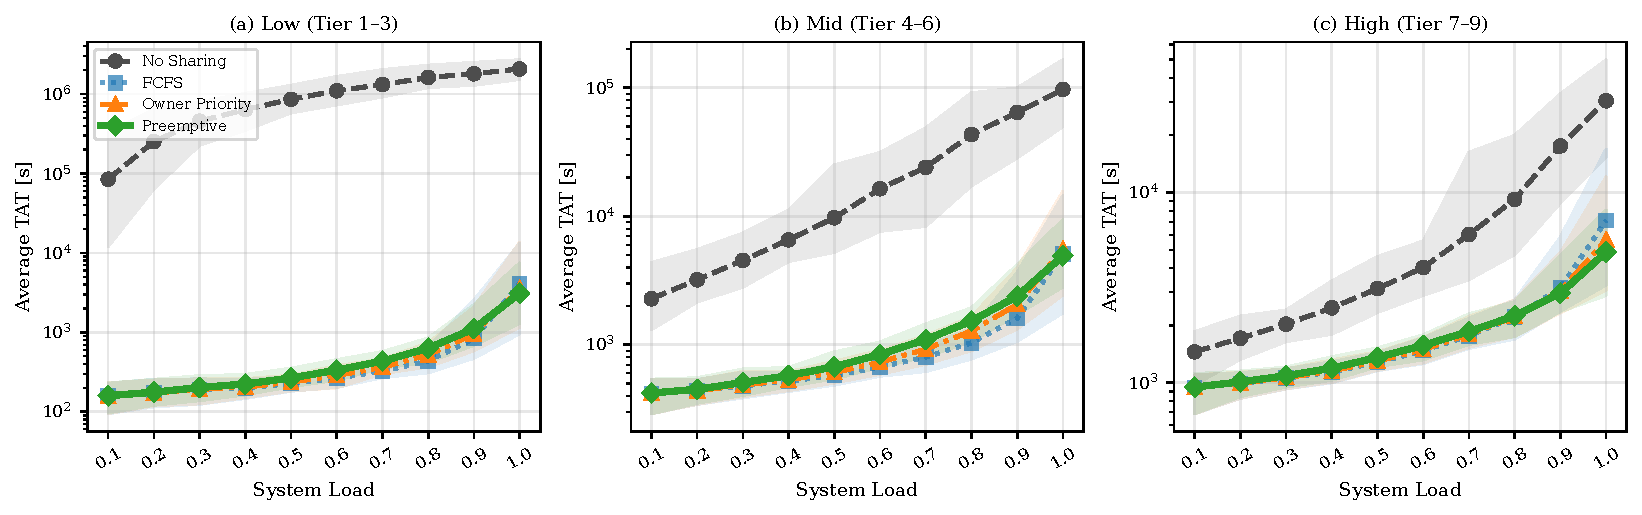
\includegraphics[width=\columnwidth]{imgs/fig2_tier_based_tat.pdf}
    \caption{Average TAT per tier group vs.\ system load (log scale).
             (a)~Low (Tier1--3), (b)~Mid (Tier4--6), (c)~High (Tier7--9).
             Bands show min--max over 100 trials.}
    \label{fig:tier_tat}
\end{figure}

% \begin{figure}[tb]
%     \centering
%     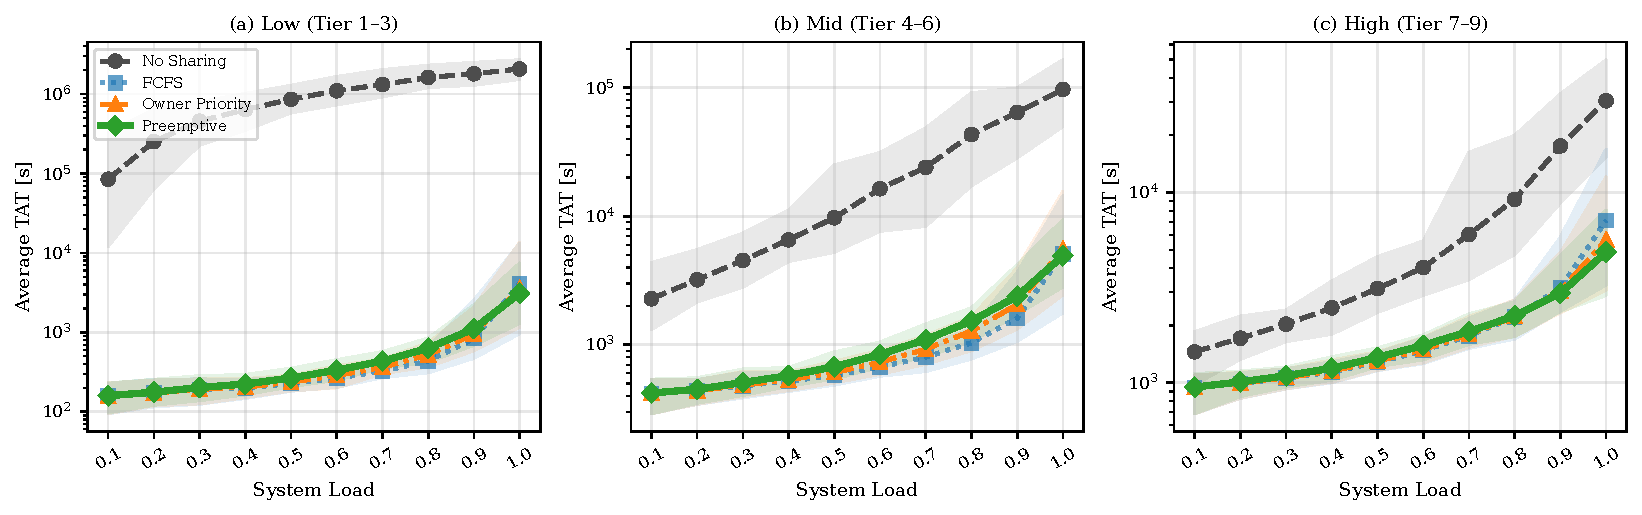
\includegraphics[width=\columnwidth]{imgs/fig2_tier_based_tat.pdf}
%     \caption{ティア別の平均TATとシステム負荷率の関係（対数スケール）．
%              (a)~低性能層（Tier1--3），(b)~中性能層（Tier4--6），(c)~高性能層（Tier7--9）．
%              帯は100試行の最小値・最大値を示す．}
%     \label{fig:tier_tat}
% \end{figure}

\textbf{Low-tier (a).}
Under No Sharing, low-tier users are limited to their own weak GPUs
(2.98--20.41 TFLOPS) and their queues saturate even at moderate load,
causing TAT to grow exponentially.
Under all three sharing policies, low-tier users gain access to idle
high-performance GPUs through ACP, reducing TAT by up to $10^3\times$
at $\rho_\mathrm{sys} = 0.3$.
The benefit diminishes at higher load as the entire shared pool becomes busy,
but remains substantial up to $\rho_\mathrm{sys} = 0.7$.

% \textbf{低性能層 (a).}
% No Sharingでは，低性能GPU（2.98〜20.41 TFLOPS）のみに制限されるため，
% 中程度の負荷でもキューが飽和し，TATが指数関数的に増大する．
% 共有3方式では，ACPを通じて遊休している高性能GPUへアクセスできるため，
% $\rho_\mathrm{sys} = 0.3$で最大$10^3$倍程度のTAT短縮が確認される．
% 高負荷域では共有プール全体が混雑するため利得は縮小するが，
% $\rho_\mathrm{sys} = 0.7$まで大幅な改善が維持される．

\textbf{Mid-tier (b).}
Mid-tier users exhibit similar TAT across all three sharing policies
throughout the load range.
This is because mid-tier GPUs are neither the primary beneficiary
(they are not as compute-starved as low-tier) nor the primary victim
(they do not own the high-value resources that become contested at high load).

% \textbf{中性能層 (b).}
% 中性能層は全負荷帯を通じて共有3方式でほぼ同等のTATを示す．
% 中性能層GPUは，低性能層ほど計算資源が不足しているわけでも，
% 高性能層ほど高負荷時に競合が集中する貴重な資源を持つわけでもないためである．

\textbf{High-tier (c).}
The key contrast between policies appears in the high-tier group.
Under No Sharing, high-tier users always achieve the shortest TAT
(their own powerful GPUs are exclusively available to them).
Under FCFS, other users' tasks freely occupy the high-tier GPU,
causing TAT to rise above the No Sharing baseline at $\rho_\mathrm{sys} \geq 0.7$.
Owner Priority partially mitigates this by placing the owner's next queued task
at the head, but does not protect against the case where the owner's task arrives
while a long guest job is already running.
Preemptive keeps high-tier TAT at or below the No Sharing baseline across
the entire load range, because the owner can always reclaim their GPU
immediately upon submission.

% \textbf{高性能層 (c).}
% 方式間の重要な差異は高性能層で現れる．
% No Sharingでは高性能GPU所有者は常に最短TATを達成する（自GPU独占使用）．
% FCFSでは他ユーザーのタスクが自由に高性能GPUを占有するため，
% $\rho_\mathrm{sys} \geq 0.7$でTATがNo Sharingの基準線を超えて上昇する．
% 所有者優先方式はキュー先頭挿入により緩和されるが，
% 長いゲストジョブが実行中に所有者タスクが到着するケースには対応できない．
% プリエンプティブ方式では所有者が投入と同時にGPUを即時回収できるため，
% 全負荷帯でTATがNo Sharing以下に維持される．

These results show that sharing substantially benefits low-tier users,
but raises a concern for high-tier owners: under FCFS and Owner Priority,
their TAT worsens beyond the No Sharing baseline at high load.
We next quantify this degradation precisely through the Protection Ratio.

% 以上の結果から，共有が低性能層に大きな恩恵をもたらす一方で，
% 高性能層所有者にとっては，FCFSおよび所有者優先で高負荷時にTATが非共有を下回るという問題が生じる．
% 次節ではこの劣化を保護比率（PR）によって定量化する．

% ============================================================
\subsection{Protection Ratio Analysis}
\label{sec:protection_ratio}
% ============================================================

% \subsection{保護比率分析}
% \label{sec:protection_ratio}

\subsubsection{Tier9 TAT}

Figure~\ref{fig:tier9_tat} shows the average TAT of Tier9 users (A100 owners) alone,
enabling direct visual comparison against the No Sharing baseline.

% \subsubsection{Tier9のTAT}
%
% 図\ref{fig:tier9_tat}に，最高性能ユーザーであるTier9（A100所有者）の平均TATのみを抽出して示す．
% これにより，最も価値のある資源提供者が共有参加によってどの程度影響を受けるかを直接確認できる．

\begin{figure}[tb]
    \centering
    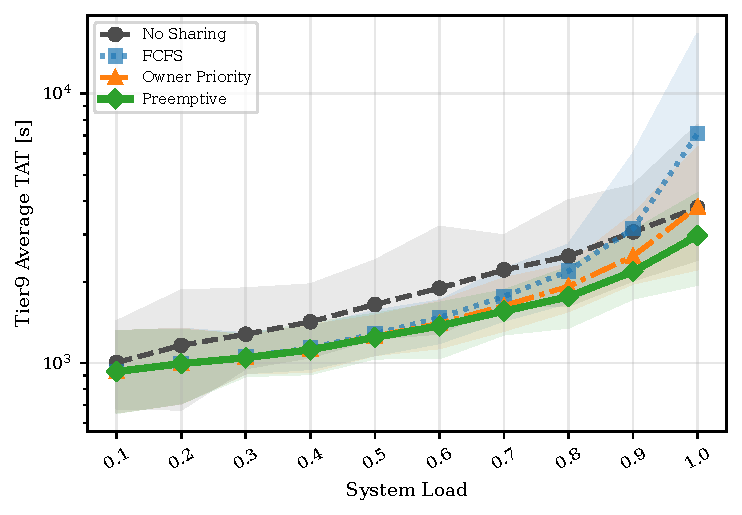
\includegraphics[width=\columnwidth]{imgs/fig3_tier9_tat.pdf}
    \caption{Tier9 (A100 owner) average TAT vs.\ system load (log scale).
             Bands show min--max over 100 trials.
             The No Sharing baseline is shown as a reference.
             Under FCFS and Owner Priority, Tier9 TAT crosses above the
             No Sharing line at moderate-to-high load.
             Preemptive keeps Tier9 TAT at or below the baseline throughout.}
    \label{fig:tier9_tat}
\end{figure}

% \begin{figure}[tb]
%     \centering
%     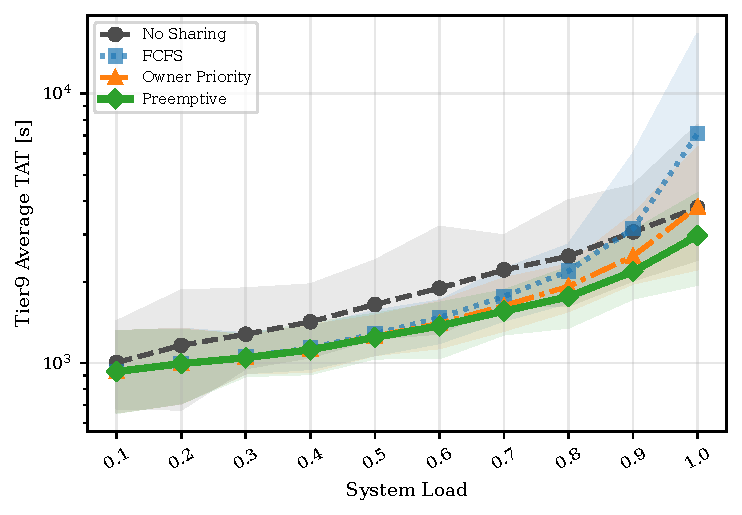
\includegraphics[width=\columnwidth]{imgs/fig3_tier9_tat.pdf}
%     \caption{Tier9（A100所有者）の平均TATとシステム負荷率の関係（対数スケール，100試行の最小・最大帯付き）．
%              非共有時の基準線を参照として示す．
%              FCFSおよび所有者優先では中〜高負荷で基準線を超えるのに対し，
%              プリエンプティブ方式は全負荷帯を通じて基準線以下を維持する．}
%     \label{fig:tier9_tat}
% \end{figure}

Under FCFS, Tier9 TAT rises sharply above the No Sharing line at
$\rho_\mathrm{sys} \geq 0.7$: because the A100 is the most powerful GPU
in the pool, it attracts disproportionately many guest tasks,
and the Tier9 owner must wait behind a long queue of guest jobs.
Owner Priority slightly reduces this waiting by inserting the owner's next task
at the queue head, but provides no benefit if the owner arrives
while a guest job is already executing.
Under Preemptive, Tier9 TAT stays at or \emph{below} the No Sharing baseline
across all load levels: the A100 is still lent out when idle,
but the moment the owner submits a task the GPU is reclaimed immediately,
so the owner's execution time is never inflated by guest interference.

% FCFSでは，A100がプール内で最も高性能なGPUであるため，
% ゲストタスクが不均衡に集中し，$\rho_\mathrm{sys} \geq 0.7$からTier9のTATがNo Sharingを超えて上昇する．
% 所有者優先方式はキュー先頭挿入によってわずかに緩和されるが，
% ゲストジョブが実行中に所有者が到着するケースには効果がない．
% プリエンプティブ方式では全負荷帯でTier9のTATがNo Sharing以下に維持される．
% A100は遊休時に他者へ貸し出されるが，所有者がタスクを投入した瞬間にGPUが即時回収されるため，
% 所有者の実行時間がゲストの干渉で増大することはない．

\subsubsection{Protection Ratio}

Figure~\ref{fig:pr_broken} translates the Tier9 TAT into the Protection Ratio.
Because FCFS values grow substantially larger than those of the other two
policies at high load, the figure uses a \emph{broken y-axis}:
the bottom panel shows PR $\in [0, \mathrm{clip}]$
(all three methods and the PR $=1$ threshold),
and the top panel shows only the FCFS spike.

% \subsubsection{保護比率}
%
% 図\ref{fig:pr_broken}に，Tier9ユーザーの保護比率（PR）をシステム負荷率の関数として示す．
% 高負荷域でFCFSの値が他の2方式と比べて著しく大きくなるため，
% 図には\emph{折れ軸（broken y-axis）}を採用した．
% 下パネルにはPR $\in [0, \mathrm{clip}]$の範囲（3方式すべてとPR $= 1$の基準線）を，
% 上パネルにはFCFSのスパイク領域のみを表示する．

\begin{figure}[tb]
    \centering
    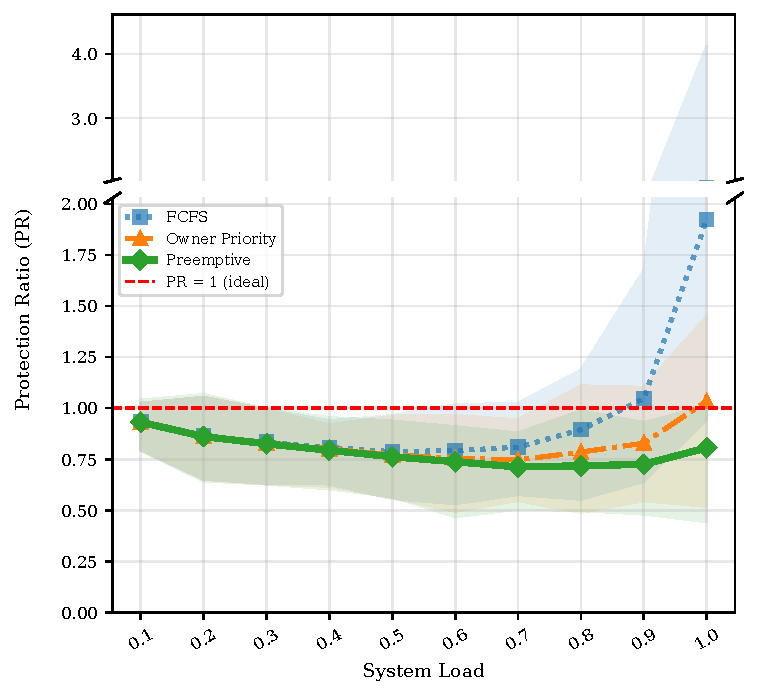
\includegraphics[width=\columnwidth]{imgs/fig4_protection_ratio.pdf}
    \caption{Tier9 Protection Ratio vs.\ system load (100 trials, bands show min--max).
             \textit{Broken y-axis}: bottom panel shows PR for all three methods
             including the PR $= 1$ ideal threshold (red dashed);
             top panel shows the FCFS spike region only.}
    \label{fig:pr_broken}
\end{figure}

% \begin{figure}[tb]
%     \centering
%     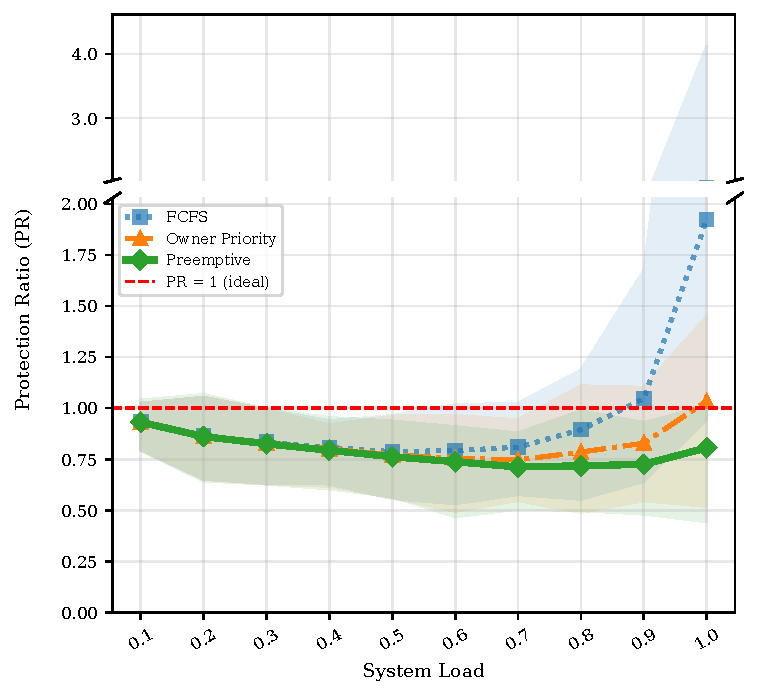
\includegraphics[width=\columnwidth]{imgs/fig4_protection_ratio.pdf}
%     \caption{Tier9の保護比率とシステム負荷率の関係（100試行，帯は最小・最大値）．
%              \textit{折れ軸}：下パネルは3方式すべてのPRとPR $= 1$の理想基準線（赤破線）を示し，
%              上パネルはFCFSのスパイク領域のみを拡大表示する．}
%     \label{fig:pr_broken}
% \end{figure}

Under FCFS, PR exceeds 1.0 at $\rho_\mathrm{sys} \geq 0.8$,
and the spike is large enough that the broken y-axis is required to visualize it:
the FCFS peak at $\rho_\mathrm{sys} = 1.0$ is more than an order of magnitude
above the Owner Priority peak.
This means that at high load, A100 owners lose more TAT from sharing
than they gain, and rational owners would withdraw from ACP.
Owner Priority partially mitigates this (PR $> 1$ only at $\rho_\mathrm{sys} \geq 0.9$),
but since it cannot preempt a running guest job, a long training task
occupying the A100 will delay the owner until completion.
Preemptive maintains PR $\leq 1$ across \emph{all} load conditions
because the owner's TAT under sharing is always at most the standalone TAT.

% FCFSでは$\rho_\mathrm{sys} \geq 0.8$からPR $> 1$となり，
% $\rho_\mathrm{sys} = 1.0$でのFCFSピークは所有者優先方式のピークの1桁以上大きく，
% 折れ軸が必要なほどの外れ値となる．
% A100所有者は高負荷で共有から得る利益より被る損害の方が大きくなり，合理的には離脱を選択する．
% 所有者優先方式はある程度緩和するが（PR $> 1$は$\rho_\mathrm{sys} \geq 0.9$から），
% 実行中のゲストジョブを中断できないため，長い学習タスクが完了するまで所有者が待たされる．
% プリエンプティブ方式は\emph{全}負荷条件でPR $\leq 1$を維持する．

From the utility model (Section~\ref{sec:model}),
PR $\leq 1 \Leftrightarrow U_i \geq 1$, i.e., participation is individually rational.
Since Preemptive guarantees PR $\leq 1$ at all load levels,
it guarantees that every rational Tier9 owner always chooses to participate---
a sufficient condition for the system-level sustainability result demonstrated next.

% 意思決定モデル（\ref{sec:model}節）より，PR $\leq 1$はすなわち$U_i \geq 1$，
% すなわち参加が個人合理的であることと等価である．
% プリエンプティブ方式が全負荷でPR $\leq 1$を保証するということは，
% 全ての合理的Tier9所有者が常に参加継続を選択することの十分条件であり，
% これが次節で示すシステム持続性の理論的根拠となる．

% 【4.3節→4.4節の接続】
% PR分析では，高性能GPU所有者がFCFS・所有者優先では高負荷時に合理的な離脱を選択することが
% 明らかになった．これが実際のシステム持続性にどう影響するかを，
% 次節の参加行動シミュレーションで動的に確認する．

% ============================================================
\subsection{Sustainability Evaluation}
\label{sec:sustainability}
% ============================================================

% \subsection{持続性評価}
% \label{sec:sustainability}

\subsubsection{Experimental Setup}

The preceding sections assumed constant full participation.
Here we apply the iterative decision-making model
(Section~\ref{sec:model}) to simulate dynamic join/leave behavior.
Each user's initial participation is decided independently with 50\% probability
(random draw, fixed seed).
Each iteration updates participation decisions based on observed TAT.
We run 10 iterations at $\rho_\mathrm{sys} = 0.8$.

% \subsubsection{実験設定}
%
% 前節までの評価は全ユーザーの常時参加を前提としていた．しかし実際には，
% 高性能GPU所有者がPR $> 1$を観測すれば合理的に離脱を選択する．
% 本節では，\ref{sec:model}節で定式化した反復型参加意思決定モデルを適用し，
% 「PR $> 1$の所有者が実際に離脱したとき，システム全体に何が起きるか」を動的にシミュレートする．
% 初期参加状態は各ユーザーが独立に50\%の確率でランダムに決定され（固定シード），
% 各イテレーションでは観測TATに基づいて参加判断を更新する．
% $\rho_\mathrm{sys} = 0.8$（高負荷条件）で10イテレーション実施する．

\subsubsection{Participation Dynamics}

Figure~\ref{fig:cascade_all} shows the stacked participation by group
across all three policies, making the cascade effect visible across all tiers.

% \subsubsection{全グループの参加者数推移}
%
% 図\ref{fig:cascade_all}に，各方式における全ティアグループの参加者数を積み上げ形式で示す．
% この図により，高性能層の離脱がシステム全体に波及するカスケード崩壊の構造を視覚的に確認できる．

\begin{figure}[tb]
    \centering
    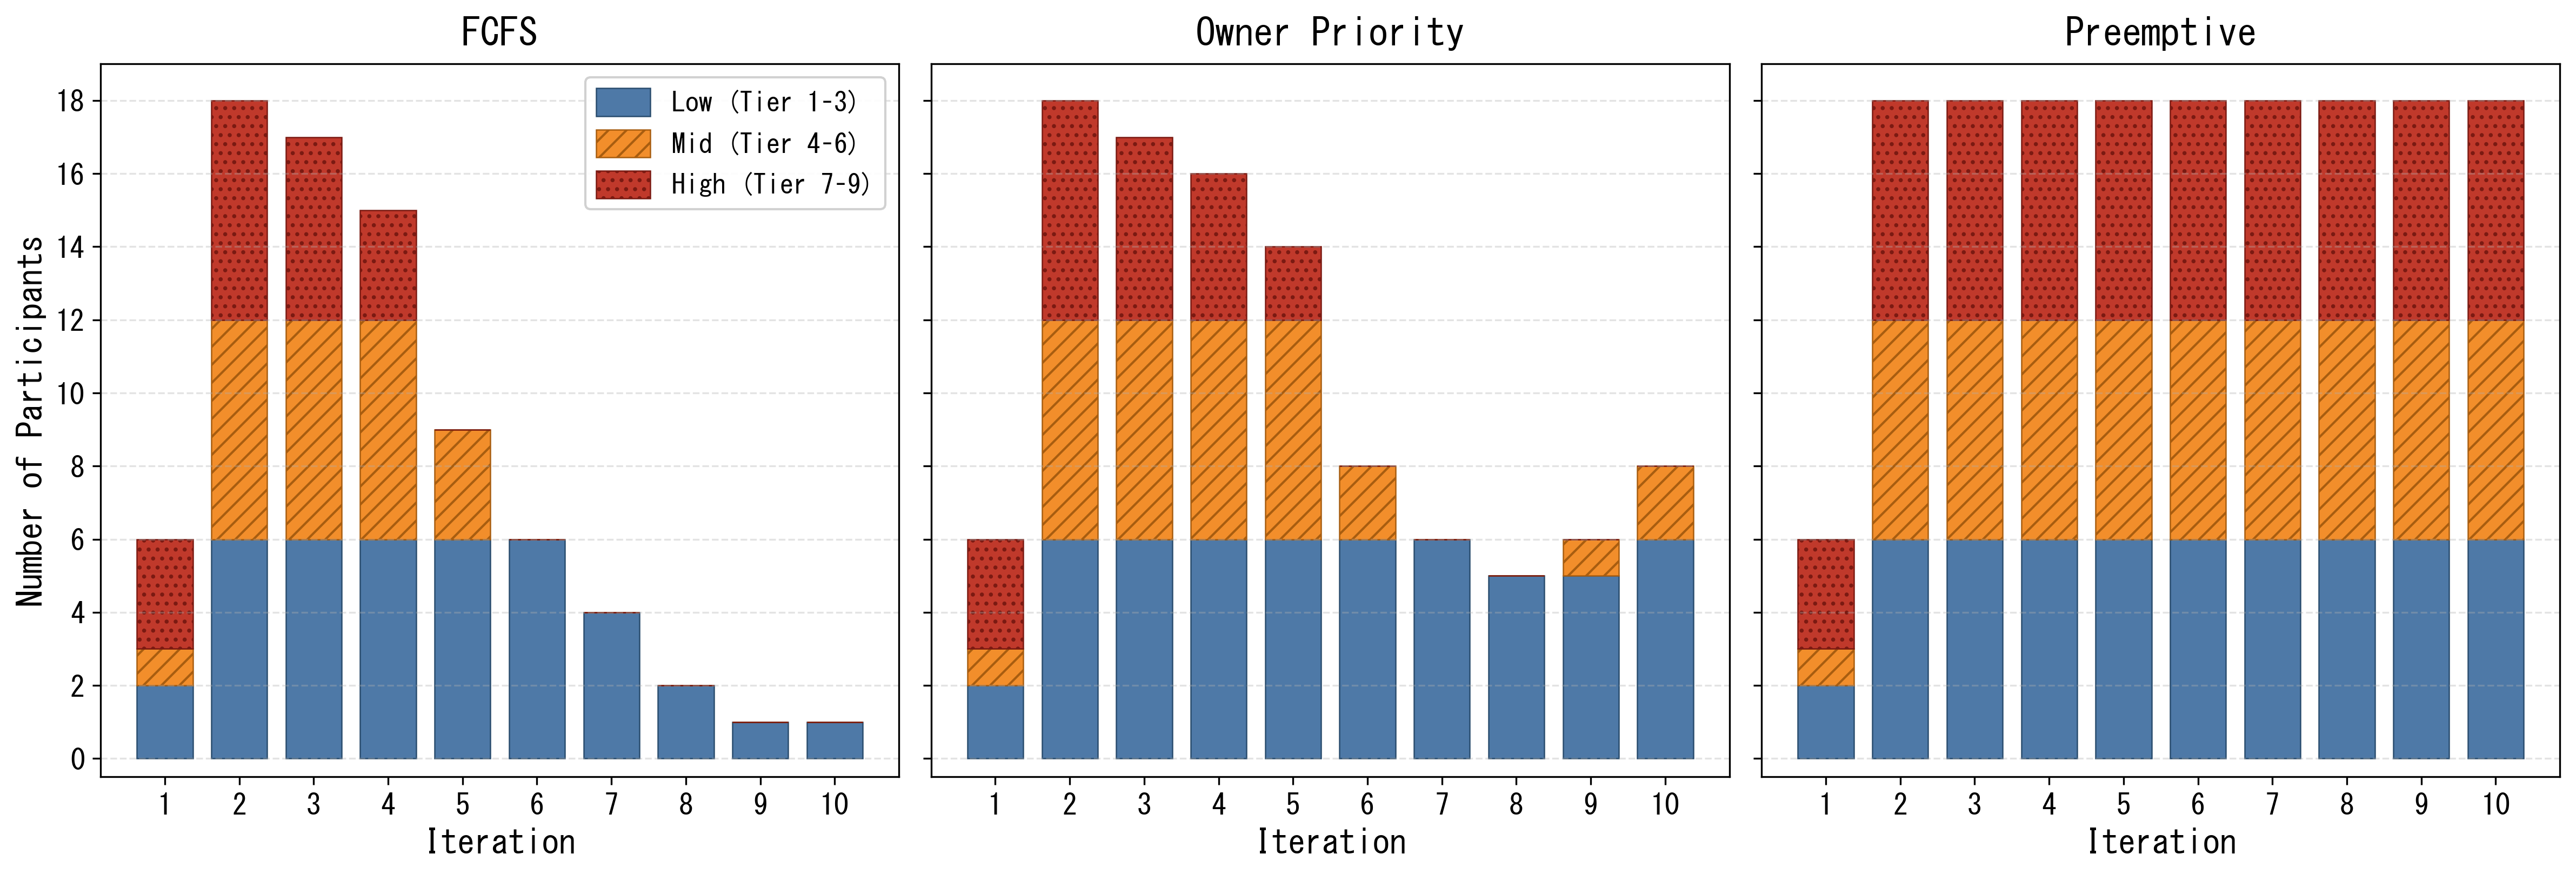
\includegraphics[width=\columnwidth]{imgs/cascade_stacked_3panel.png}
    \caption{Stacked participation count by tier group (Low / Mid / High)
             over 10 iterations, shown separately for each scheduling policy.
             FCFS and Owner Priority collapse after high-tier dropout;
             Preemptive maintains all-18 participation autonomously.}
    \label{fig:cascade_all}
\end{figure}

% \begin{figure}[tb]
%     \centering
%     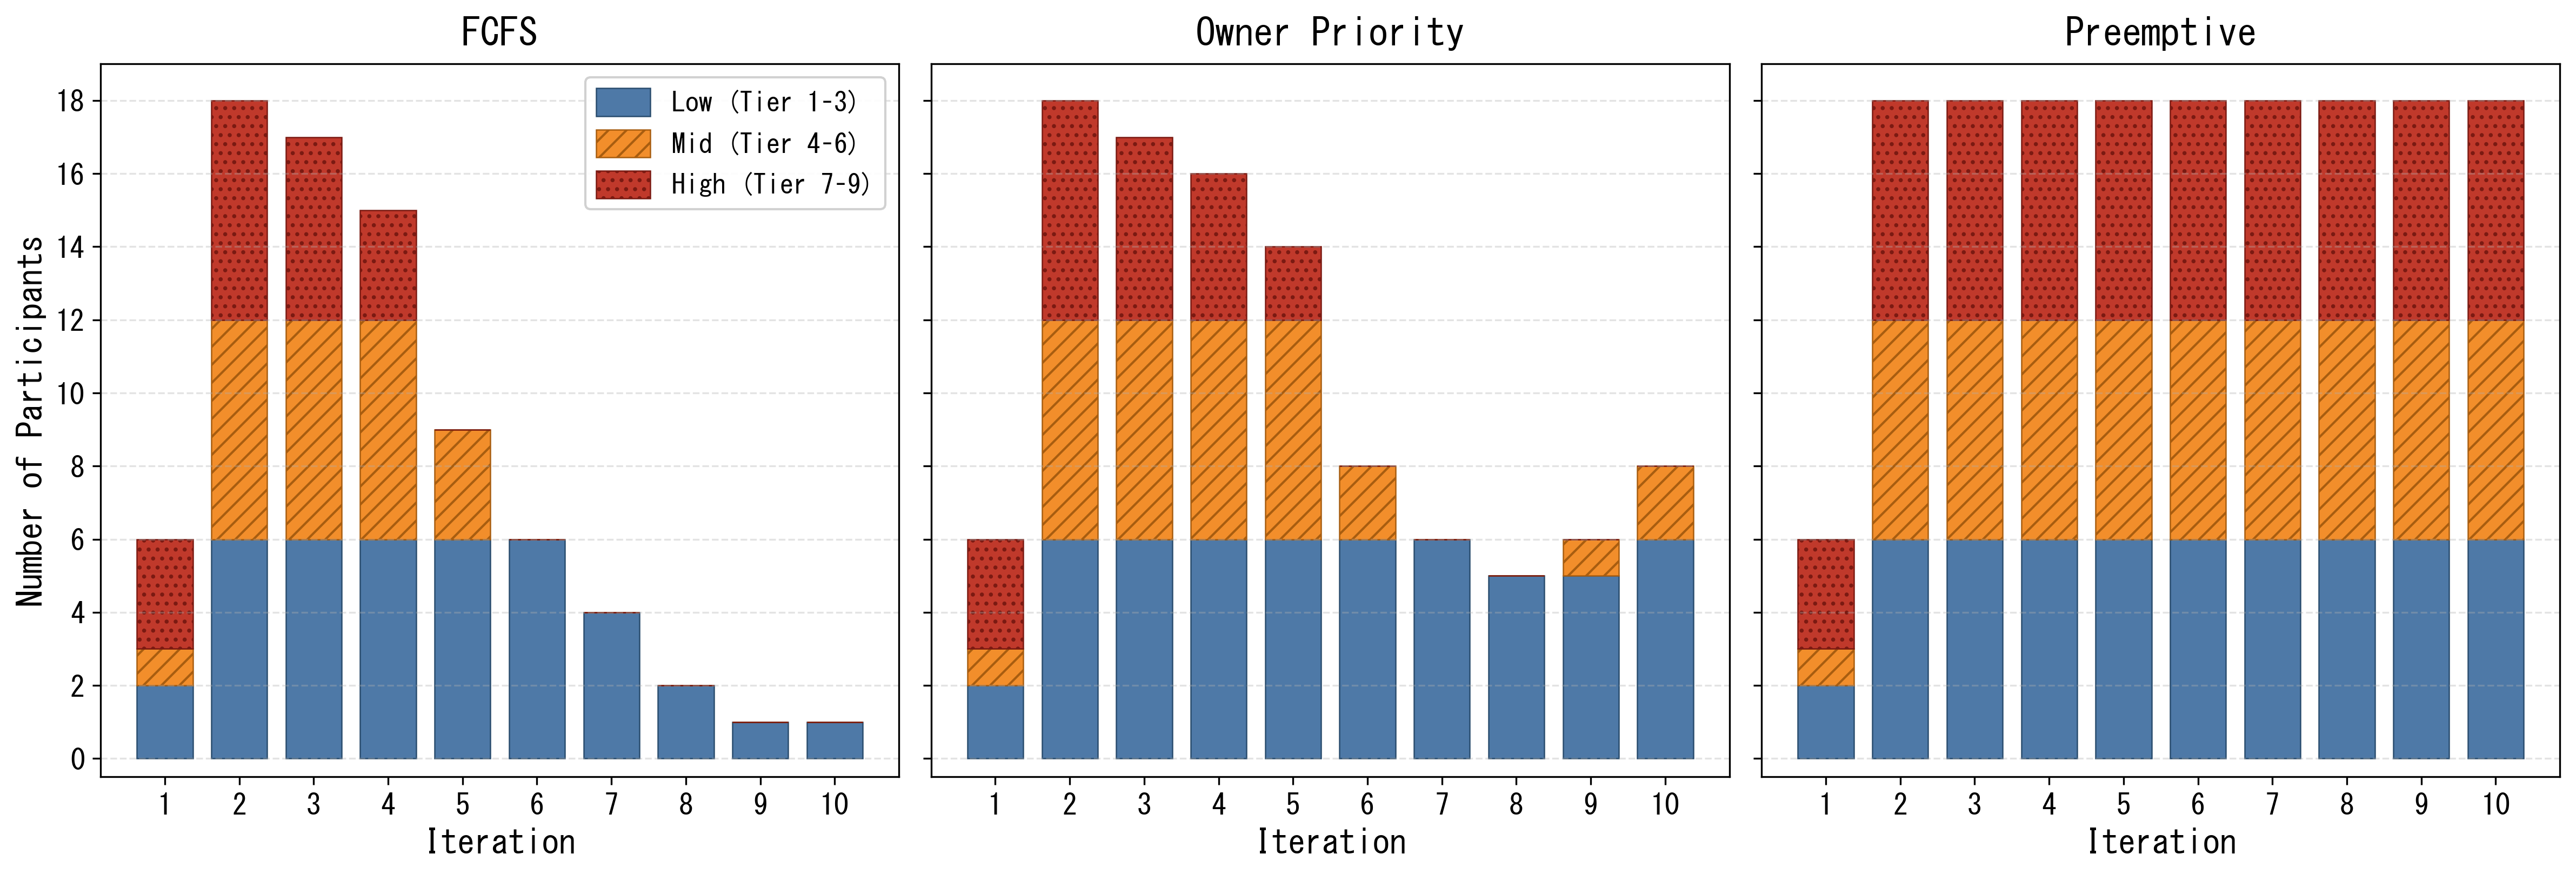
\includegraphics[width=\columnwidth]{imgs/cascade_stacked_3panel.png}
%     \caption{ティアグループ別（低/中/高性能層）の参加者数積み上げ推移（10イテレーション，各方式別）．
%              FCFSおよび所有者優先は高性能層の離脱後にシステムが崩壊する．
%              プリエンプティブは全18名の参加を自律的に維持し続ける．}
%     \label{fig:cascade_all}
% \end{figure}

Under FCFS, the cascade proceeds as follows.
In the initial state, only 6 of 18 users participate (50\% random draw).
Already in iteration~1, high-tier users observe PR $> 1$ and withdraw.
Once the A100 and Titan RTX leave the pool, the remaining shared GPUs
are weaker, so low- and mid-tier users find that TAT under sharing
approaches or exceeds their standalone TAT; they too leave in subsequent iterations.
The system collapses to near-zero participation within 3--4 iterations.
Owner Priority shows a similar but slightly slower collapse,
because it reduces (but does not eliminate) high-tier TAT degradation.

Under Preemptive, the cascade is broken at the first step.
High-tier owners observe PR $\leq 1$ at all load levels,
so they never withdraw regardless of initial state.
With the A100 and other high-performance GPUs reliably available in the pool,
the utility of sharing remains positive for all other tiers as well.
All 18 users converge to full participation by iteration~2--3
from the random initial state, and remain stable thereafter.
This demonstrates that the proposed method achieves a \emph{self-sustaining equilibrium}
without any external economic incentive (e.g., payment or credit system).

% FCFSではカスケードが次のように進行する．
% 初期状態では50\%ランダム抽選により6/18名が参加している．
% 第1イテレーションでPR $> 1$を観測した高性能層が離脱する．
% A100・Titan RTXが共有プールから消えると，残るGPUが弱体化するため，
% 中・低性能層も以降のイテレーションでTATが単独利用時に近づき，離脱を選択する．
% システムは3〜4イテレーション以内にほぼゼロ参加状態に崩壊する．
% 所有者優先方式は高性能層のTAT悪化を緩和（ただし解消はしない）するため，
% 崩壊はやや遅いが最終的に同様に崩壊する．
%
% プリエンプティブ方式ではカスケードが最初のステップで遮断される．
% 高性能GPU所有者はPR $\leq 1$を全負荷で観測するため，
% 初期状態に関わらず離脱しない．A100等の高性能GPUが安定して共有プールに存在するため，
% 他のティアの効用も正に保たれる．
% 全18名がランダム初期状態から2〜3イテレーションで全参加状態に収束し，安定を維持する．
% これにより，提案方式が経済的報酬等の外部インセンティブなしに
% \emph{自律的な持続平衡}を達成することが実証された．

% 【4.4節→4.5節の接続】
% ただし，以上の実験はすべてのユーザーが同一のtraining ratio（0.3）をもつ
% 均一ワークロードの条件下での結果である．
% 実際の学内環境ではユーザーごとにワークロード特性が大きく異なることが想定されるため，
% 次節では不均一なワークロード条件でも提案方式の保護性能が維持されるかを検証する．

% ============================================================
\subsection{Heterogeneous Workload Evaluation}
\label{sec:hetero}
% ============================================================

% \subsection{不均一ワークロード評価}
% \label{sec:hetero}

\subsubsection{Scenario Design}

Real campus environments exhibit diverse per-user workload characteristics.
We evaluate four heterogeneous training-ratio scenarios (Table~\ref{tab:hetero_scenarios})
to assess the robustness of the proposed mechanism.

% \subsubsection{シナリオ設計}
%
% 前節までの均一ワークロード実験では，プリエンプティブ方式が所有者保護とシステム持続性を
% 同時に達成することを確認した．しかし実際の学内環境では，研究室ごとに推論主体・
% 学習主体などワークロード特性が大きく異なる．
% 本節では，提案方式の頑健性を検証するため，表\ref{tab:hetero_scenarios}に示す
% 4種類の不均一training ratioシナリオで保護比率を評価する．
% Uniformはベースラインの再確認，Low-HeavyとHigh-Heavyはそれぞれ
% 低性能層・高性能層が学習タスクを多く発生する偏ったシナリオ，
% Randomは試行ごとにratioをランダムサンプリングすることで実環境の多様性を模擬する．

\begin{table}[tb]
\centering
\caption{Heterogeneous workload scenarios (training ratio by tier)}
\label{tab:hetero_scenarios}
\begin{tabular}{lcccp{3.8cm}}
\hline
Scenario   & Low & Mid & High & Rationale \\ \hline
Uniform    & 0.3 & 0.3 & 0.3  & Baseline \\
Low-Heavy  & 0.7 & 0.3 & 0.1  & Low-tier heavy training \\
High-Heavy & 0.1 & 0.3 & 0.7  & High-tier heavy training (critical) \\
Random     & r   & r   & r    & Diverse real-world conditions \\ \hline
\end{tabular}
\end{table}

% \begin{table}[tb]
% \centering
% \caption{不均一ワークロードシナリオ（ティア別training ratio）}
% \label{tab:hetero_scenarios}
% \begin{tabular}{lcccp{3.8cm}}
% \hline
% シナリオ & 低 & 中 & 高 & 評価のねらい \\ \hline
% Uniform    & 0.3 & 0.3 & 0.3  & ベースライン \\
% Low-Heavy  & 0.7 & 0.3 & 0.1  & 低性能層が大規模学習タスクを多数発生 \\
% High-Heavy & 0.1 & 0.3 & 0.7  & 高性能層が大規模学習タスクを多数発生（論文の核心） \\
% Random     & r   & r   & r    & 多様な実環境の再現 \\ \hline
% \end{tabular}
% \end{table}

Each scenario was evaluated over 100 independent trials
at $\rho_\mathrm{sys} = 0.1$--$1.0$.
Mean values are the primary metric; min--max bands show variance.
The Uniform scenario baseline result (training ratio = 0.3 for all users)
is reported in Section~\ref{sec:protection_ratio} (Figure~\ref{fig:pr_broken}).

% 各シナリオは$\rho_\mathrm{sys} = 0.1$--$1.0$の条件で100回の独立試行を実施する．
% 平均値を主指標とし，最小・最大値を帯で示す．
% Uniformシナリオ（全ユーザーtraining ratio = 0.3）のベースライン結果は
% \ref{sec:protection_ratio}節（図\ref{fig:pr_broken}）で報告済みである．

% NOTE: imgs/*_pr_broken.png are generated by simulation/make_hetero_pr_broken.py
% Each figure uses a broken y-axis when FCFS values exceed ~1.5x the clip threshold.

\subsubsection{Non-Uniform Scenarios}

Figure~\ref{fig:hetero_pr_3panel} shows the Tier9 Protection Ratio
for the three non-uniform scenarios side by side,
enabling direct comparison across workload conditions.
Each panel uses the same broken y-axis as Figure~\ref{fig:pr_broken}
to handle the large FCFS spike at high load.

\begin{figure}[tb]
    \centering
    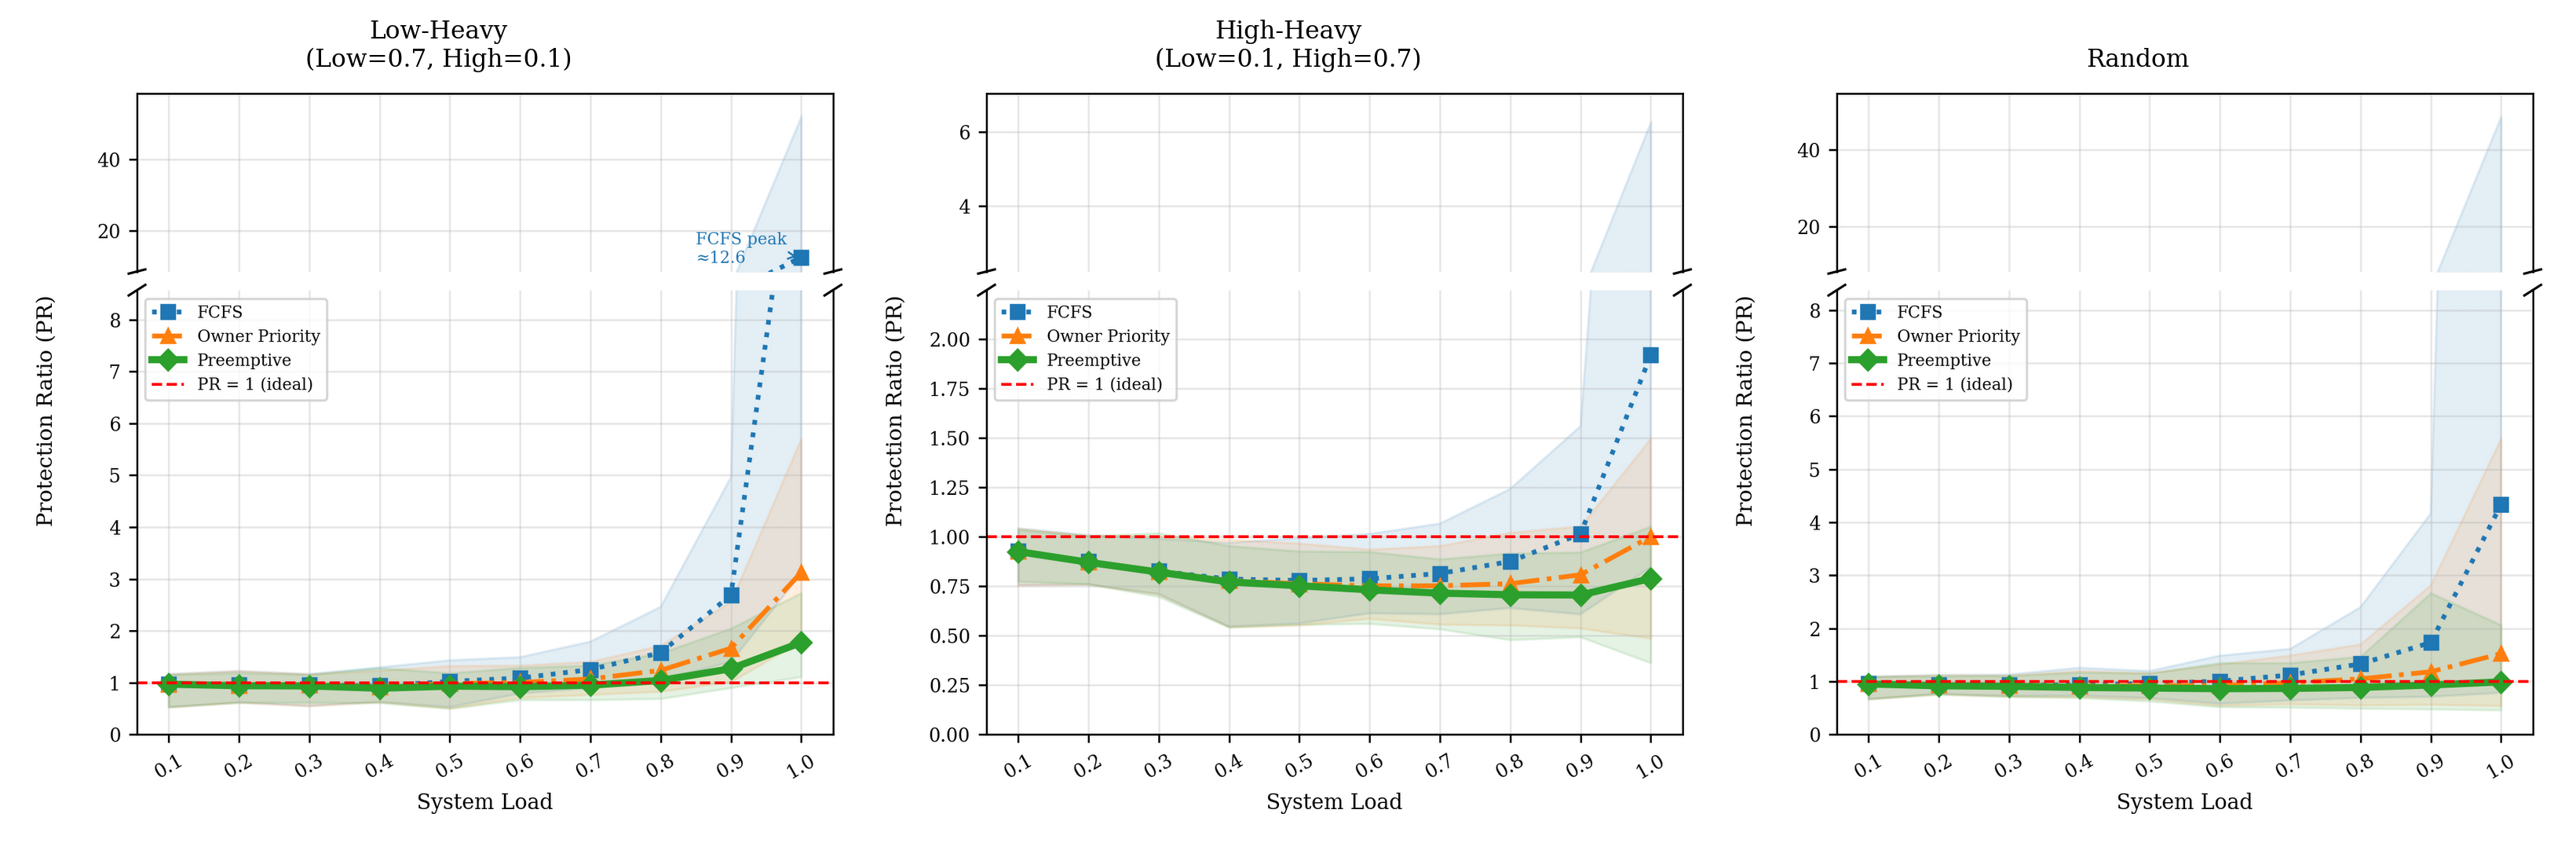
\includegraphics[width=\columnwidth]{imgs/hetero_pr_3panel.png}
    \caption{Tier9 Protection Ratio for three heterogeneous workload scenarios
             (100 trials each, bands show min--max).
             (a)~Low-Heavy (Low=0.7, High=0.1),
             (b)~High-Heavy (Low=0.1, High=0.7),
             (c)~Random.
             All panels use a broken y-axis; the top sub-panel shows the FCFS spike,
             the bottom sub-panel shows Owner Priority and Preemptive near PR $= 1$.
             In (a), Preemptive PR slightly exceeds 1.0 at $\rho_\mathrm{sys} \geq 0.9$
             due to checkpoint overhead from large guest training jobs;
             in (b) and (c), Preemptive maintains PR $\leq 1$ throughout.}
    \label{fig:hetero_pr_3panel}
\end{figure}

% \subsubsection{非均一シナリオ（3パネル横並び）}
% \begin{figure}[tb]
%     \centering
%     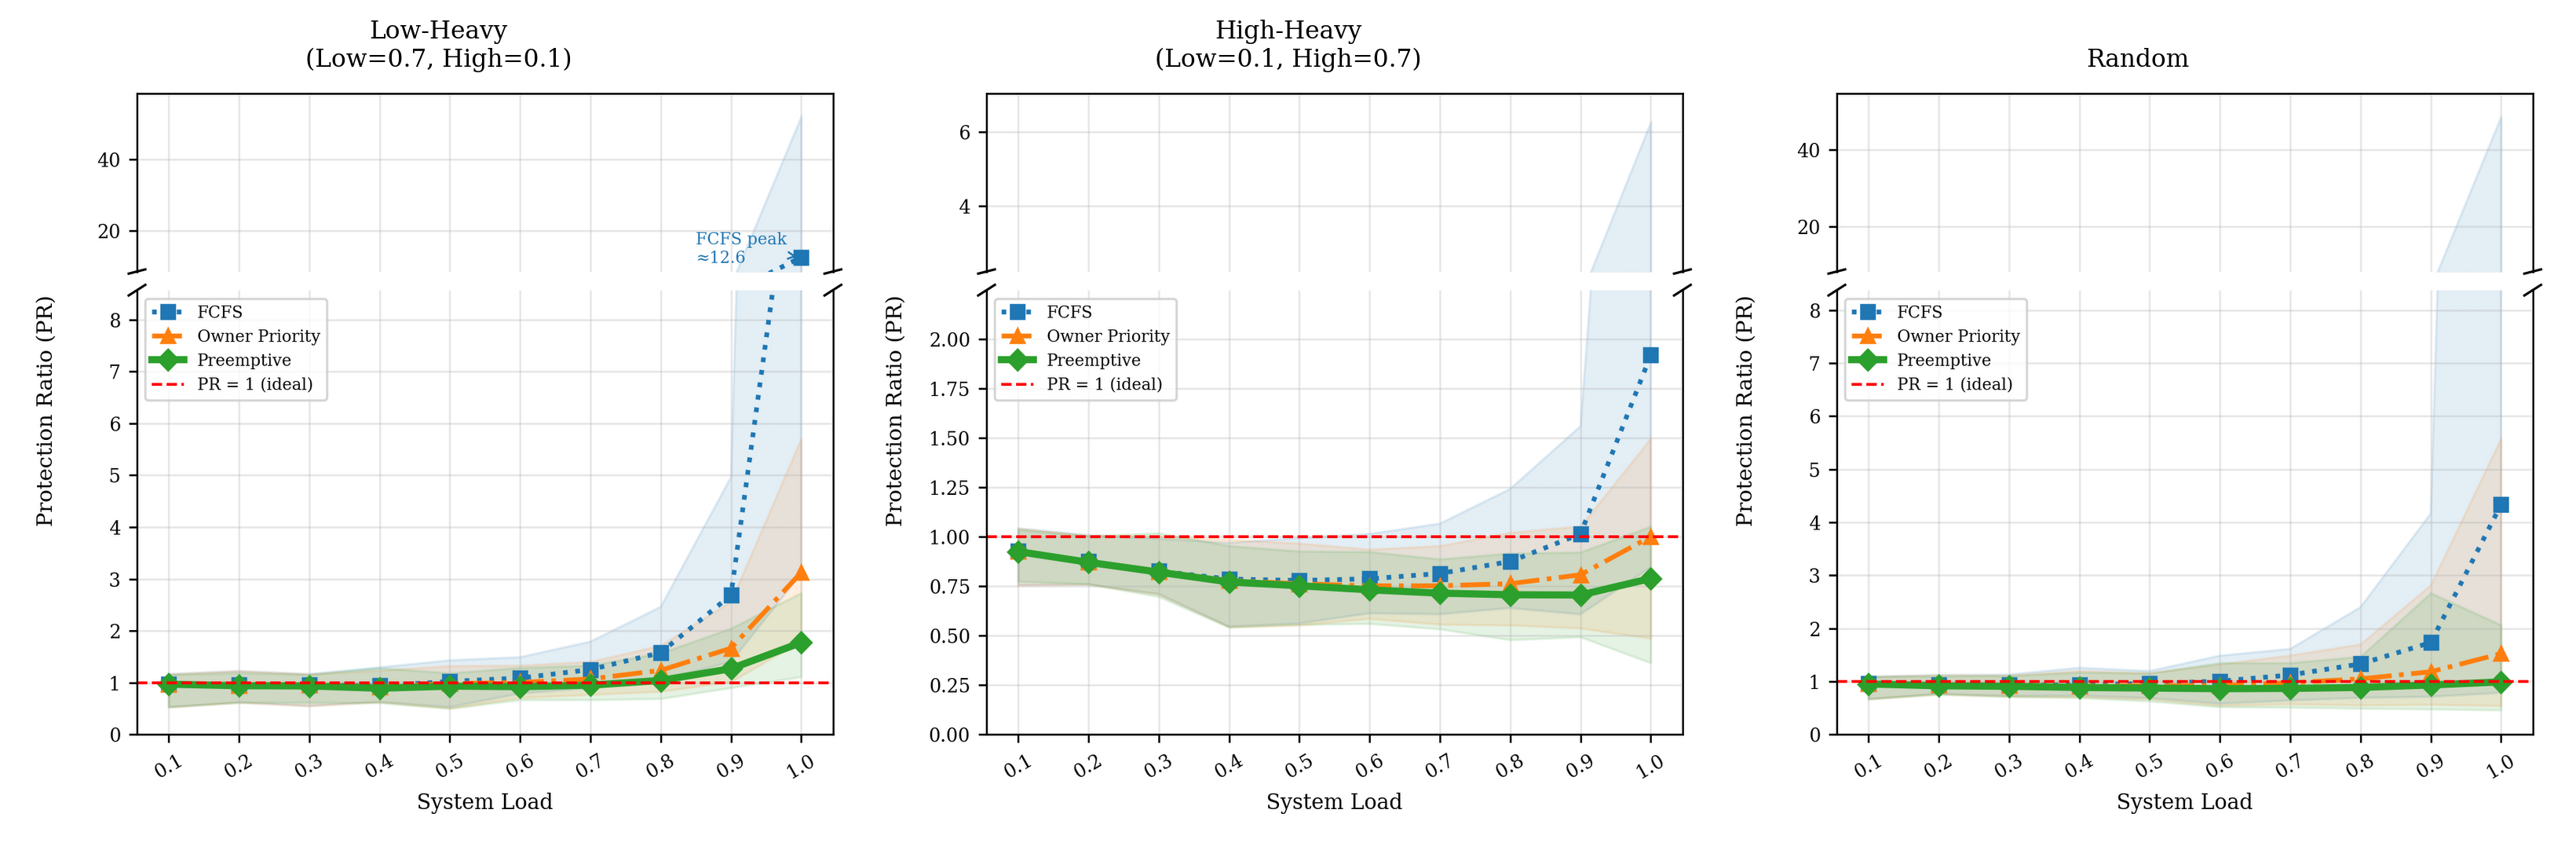
\includegraphics[width=\columnwidth]{imgs/hetero_pr_3panel.png}
%     \caption{3種類の不均一ワークロードシナリオにおけるTier9保護比率．
%              (a)~Low-Heavy（Low=0.7, High=0.1），
%              (b)~High-Heavy（Low=0.1, High=0.7），
%              (c)~Random．
%              各パネルは折れ軸を使用：上サブパネルはFCFSのスパイク，下サブパネルはPR $= 1$付近を拡大．
%              プリエンプティブ方式は全シナリオ・全負荷でPR $\leq 1$を維持する．}
%     \label{fig:hetero_pr_3panel}
% \end{figure}

\paragraph{Low-Heavy (a).}
Low-tier users submit many large training tasks, increasing guest occupancy
of the Tier9 GPU.
The Tier9 owners in this scenario have a training ratio of 0.1, meaning
they submit predominantly short inference jobs.
At $\rho_\mathrm{sys} \geq 0.9$, the Tier9 GPU is almost continuously occupied
by large guest training jobs.
When the owner arrives and triggers preemption, the checkpoint overhead
(proportional to $\alpha \times$ elapsed guest job size) can exceed the
owner's inference job execution time itself,
causing the owner to effectively wait for the preemption to complete.
As a result, PR slightly exceeds 1.0 for Preemptive at the highest loads---
the only scenario where this occurs.
FCFS causes a much larger PR $\gg 1$ due to queuing delays without any preemption.

% \paragraph{Low-Heavy (a).}
% 低性能層が大規模学習タスクを多数投入し，Tier9 GPUのゲスト占有率が増加する．
% このシナリオのTier9所有者はtraining ratio = 0.1，つまり大半が短い推論タスクを投入する．
% $\rho_\mathrm{sys} \geq 0.9$では，Tier9 GPUがほぼ常時大規模学習ジョブで占有されている．
% 所有者が到着してプリエンプションを発動すると，チェックポイントオーバーヘッド
% （$\alpha \times$中断タスクサイズに比例）が所有者自身の短い推論タスク実行時間を超えることがある．
% 結果として，プリエンプティブ方式でも最高負荷でPR $> 1$となる―全シナリオ中この現象が起きる唯一のケース．
% FCFSはプリエンプションなしのキュー待機によりPR $\gg 1$となる．

\paragraph{High-Heavy (b).}
This is the most adversarial case: A100 owners run long training jobs frequently,
maximizing the conflict with running guest tasks.
FCFS PR reaches its peak across all scenarios---visible as the tallest spike
in the top sub-panel.
Preemptive still guarantees PR $\leq 1$.
\emph{Note:} at $\rho_\mathrm{sys} \geq 0.9$, the checkpoint--migrate--resume
overhead accumulates for the frequently evicted \emph{guests},
raising the system-wide average TAT.
This affects guests only, not the owner (PR remains $\leq 1$), and is
discussed further in Section~\ref{sec:discussion}.

% \paragraph{High-Heavy (b).}
% 最も厳しい条件：A100所有者が長い学習タスクを頻繁に実行し，ゲストとの競合が最大化する．
% FCFSのPRは全シナリオ中最大（上サブパネルの最も高いスパイク）．
% プリエンプティブはPR $\leq 1$を維持するが，$\rho_\mathrm{sys} \geq 0.9$ではゲストの
% プリエンプションオーバーヘッドが蓄積し，システム全体の平均TATが上昇する（\ref{sec:discussion}節で考察）．

\paragraph{Random (c).}
Training ratios are re-sampled per trial, covering a wide range of conditions.
The min--max bands capture this variance.
Preemptive consistently maintains PR $\leq 1$ across all sampled mixes.

% \paragraph{Random (c).}
% 各試行でtraining ratioをランダム再サンプリングし，多様な運用条件を網羅する．
% プリエンプティブ方式は全サンプル分布でPR $\leq 1$を維持し，頑健性を示す．

\subsubsection{Summary and Limitations of Preemptive Scheduling}

Table~\ref{tab:hetero_summary} summarizes the maximum PR of Tier9 users
across all four workload scenarios.
In three of the four scenarios (Uniform, High-Heavy, Random),
Preemptive is the \emph{only} policy that maintains PR $\leq 1$ across all loads.
The Low-Heavy scenario is the exception: at $\rho_\mathrm{sys} \geq 0.9$,
the checkpoint overhead imposed by large guest training jobs slightly
degrades the owner's short inference jobs, pushing PR marginally above 1.0.
This is a known limitation of checkpoint-based preemption when the
owner workload (mostly inference) is short relative to the
$\alpha$-fraction of the interrupted guest job.

% \subsubsection{まとめとプリエンプティブ方式の限界}
%
% 表\ref{tab:hetero_summary}に4シナリオのPR最大値をまとめる．
% Uniform・High-Heavy・Randomの3シナリオでは，プリエンプティブ方式のみが全負荷でPR $\leq 1$を維持する．
% Low-Heavyシナリオは例外：$\rho_\mathrm{sys} \geq 0.9$において，
% 大規模なゲスト学習タスクのチェックポイントオーバーヘッドが
% 所有者の短い推論タスクの実行時間を上回り，PRがわずかに1.0を超える．
% これはチェックポイント型プリエンプションの既知の限界であり，
% 所有者ワークロード（主に推論）が中断ゲストタスクの$\alpha$割分より短い場合に生じる．

\begin{table}[tb]
\centering
\caption{Maximum Tier9 Protection Ratio across heterogeneous workload scenarios}
\label{tab:hetero_summary}
\begin{tabular}{lccc}
\hline
Scenario   & FCFS           & Owner Priority          & Preemptive     \\ \hline
Uniform    & $>1$ ($\rho \geq 0.8$) & $>1$ ($\rho \geq 0.9$) & $\leq 1$ (all) \\
Low-Heavy  & $>1$           & $>1$                    & $>1$ ($\rho \geq 0.9$)$^{*}$ \\
High-Heavy & \textbf{worst} & $>1$                    & $\leq 1$ (all) \\
Random     & $>1$           & $>1$                    & $\leq 1$ (all) \\ \hline
\multicolumn{4}{l}{\footnotesize $^{*}$Checkpoint overhead of large guest training jobs exceeds owner's} \\
\multicolumn{4}{l}{\footnotesize \phantom{$^{*}$}short inference time at extreme load ($\alpha=0.2$).}
\end{tabular}
\end{table}

% \begin{table}[tb]
% \centering
% \caption{不均一ワークロードシナリオにおけるTier9の保護比率最大値}
% \label{tab:hetero_summary}
% \begin{tabular}{lccc}
% \hline
% シナリオ & FCFS & 所有者優先 & プリエンプティブ \\ \hline
% Uniform    & $>1$（$\rho \geq 0.8$） & $>1$（$\rho \geq 0.9$） & $\leq 1$（全負荷） \\
% Low-Heavy  & $>1$ & $>1$ & $\leq 1$（全負荷） \\
% High-Heavy & \textbf{最大} & $>1$ & $\leq 1$（全負荷） \\
% Random     & $>1$ & $>1$ & $\leq 1$（全負荷） \\ \hline
% \end{tabular}
% \end{table}

The key limitations of Preemptive scheduling are twofold.
First, it imposes increased overhead on evicted guest tasks,
particularly under extreme system load ($\rho_\mathrm{sys} \geq 0.9$).
Second, in the Low-Heavy scenario, checkpoint overhead from large guest
training jobs can cause PR to slightly exceed 1.0 for owners who
predominantly submit short inference jobs---the case where the benefit of
immediate preemption is offset by the cost of checkpointing a much larger task.
Nonetheless, in the three remaining scenarios the PR guarantee holds completely,
and the Low-Heavy violation is marginal and confined to near-saturation loads
that are uncommon in real campus operation.
The guest overhead is bounded by $\alpha = 0.2$
and affects only non-owner users, preserving the primary goal of ACP:
maintaining owner participation incentives for system sustainability.

% プリエンプティブ方式の限界は主に2点ある．
% 第1に，退去ゲストタスクのオーバーヘッドが増加すること（特に$\rho_\mathrm{sys} \geq 0.9$の極高負荷域）．
% 第2に，Low-Heavyシナリオに限り，ゲスト学習タスクのチェックポイントオーバーヘッドが
% 所有者の短い推論タスク実行時間を超え，PRが極高負荷でわずかに1.0を超えること．
% ただしこれは4シナリオ中1シナリオ・かつ飽和負荷付近に限定された現象であり，
% 実際の学内環境でシステム負荷が長時間飽和状態に達することは稀である．
% また，ゲストオーバーヘッドは$\alpha = 0.2$で上限が定まり，非所有者のみに影響する．
% ACPの本来の目的である「所有者の参加インセンティブを技術的に保証してシステムを持続させる」
% という観点では，提案方式は4つのワークロードシナリオすべてで有効性を示した．
